\documentclass{article}
\usepackage{listings}
\usepackage{graphicx}
\graphicspath{{"D:\Courses\STAT S 670\Homework1"}}
\begin{document}
\lstset{language=R}
\centerline{\sc \large STAT S 670 Exploratory Data Analysis - Homework \#1}
\vspace{.5pc}
\centerline{\sc Ganesh Nagarajan}
\centerline{\it gnagaraj@indiana.edu}
\vspace{2pc}
\section{Solutions}
\begin{enumerate}
\item Following is the R code to plot the given bivariate function $f(x,y)=cos(x)sin(y)$,
\lstinputlisting[language=R]{test.R}
For the sample input,
\begin{lstlisting}
plot3d(1:10,1:10)
\end{lstlisting}
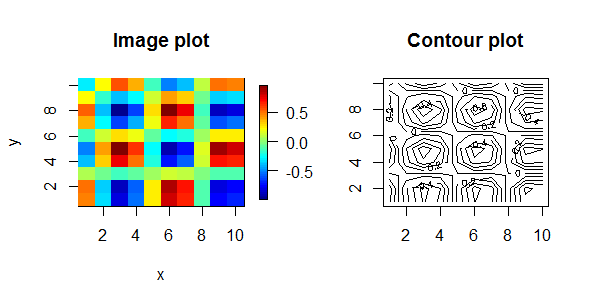
\includegraphics[scale=0.5]{perspplot1}
\\This function takes two vectors xVector and yVector as arguments which are in turn used to plot the perspective plot. It also checks if the length of xVector is equal to yVector to maintain consistency for the plot.
\item The arrows point to the gradient can be given as follows,\\
\begin{lstlisting}
plot3dDerivative(1:10,1:10)
\end{lstlisting}
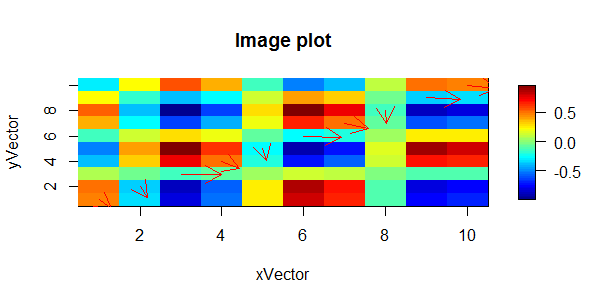
\includegraphics[scale=0.5]{derivplot}
\item Stem and Leaf plots
\begin{enumerate}
\item
\begin{enumerate}
\item
For problem 2(c) Following is the manual calculation of stem leaf plots.
\begin{center}
\begin{tabular}{|c  |c  |c|}
$Depths$ & $Stem$ & $Leaves$ \\ \hline
2&	3.&	6 8\\
4&4*&1 2\\
6&4.&9 9\\
8&5*&0 1\\
10&5.&5 5\\
(2)&6*& 3 3\\
9&7*&1 3\\
7&7.&6 9\\
5&8.&6 8\\
3&9.&0 9\\
1&10*&1\\ \hline
\end{tabular}
\end{center}
The above dataset need not be presented by the two stem per leaves model. The Dataset even if represented by normal scale it would not have been cluttered.
\item
\lstinputlisting[language=R]{stemleafplot.R}
\begin{enumerate}
\item For scale 0.25, output is as follows,\\
The decimal point is 1 digit(s) to the left of the $|$\\
  0 $|$ 8999\\
  1 $|$ 01222233344455556
\item For scale 0.5, output is as follows,\\
The decimal point is 1 digit(s) to the left of the $|$\\

  0 $|$ 8999\\
  1 $|$ 012222333444\\
  1 $|$ 55556\\
\item For scale 1, output is as follows,\\
The decimal point is 2 digit(s) to the left of the $|$\\

  08 $|$ 0000\\
  10 $|$ 00\\
  12 $|$ 0000000\\
  14 $|$ 0000000\\
  16 $|$ 0\\
\item In this data set, scale 1 looses its accuracy, since would not be appropriate to represent the data.Scale of 0.25 is way too crowded for interpretation. By the rules, a two stem per leaf would be well appropriate for representing data and the scale of 0.5 would represent this in a concise manner.By the Rule, since n $<$ 100, $2\sqrt{21}$ rule can be used. Thus 9 stems are allowed and in all three scales, the stems have doesn't than 9 stems and hence is allowed allowed by the rule.
\end{enumerate}
\item This section describes the nature of distribution.
\begin{enumerate}
\item for 2(b) considering the scale of 0.5, the distribution seems to be near normal, mean is 0.1242857, median = 0.13. There are no outliers to the data set. The data set is almost symmetrical through the median. By the Rule, since n $<$ 100, $2\sqrt{n}$ rule can be used. Thus 9 stems are allowed and in all three scales. Since the stems are more than 9, the scale wouldn't be appropriate and not allowed by the rule.
\item for 2(c), from the manually calculated stem leaf plot, there are no outliers and the data is equally distributed in all frequency. The data is almost symmetrical, however a skew is observed in the 10* portion of the stem leaf plot.
\end{enumerate}
\end{enumerate}
\end{enumerate}
\item rgamma function and Kernel Density Estimates.\\The R code for all plots in $4$ question is as follows,
\lstinputlisting[language=R]{qqplot1.R}
\begin{enumerate}
\item Following is the exact density function for DataSet1 and DataSet2\\
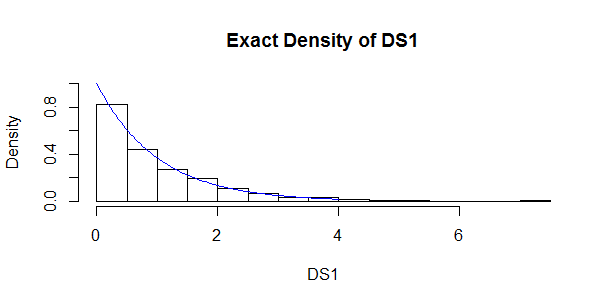
\includegraphics[scale=0.5]{curve1}
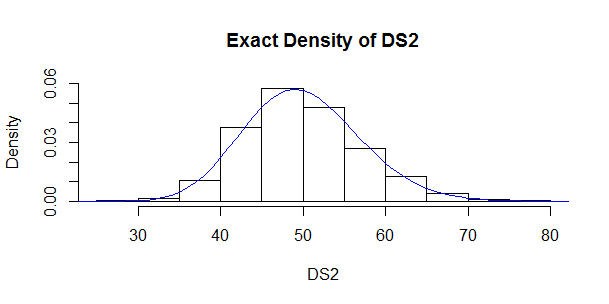
\includegraphics[scale=0.5]{curve2}
\item The QQ plot is as follows\\
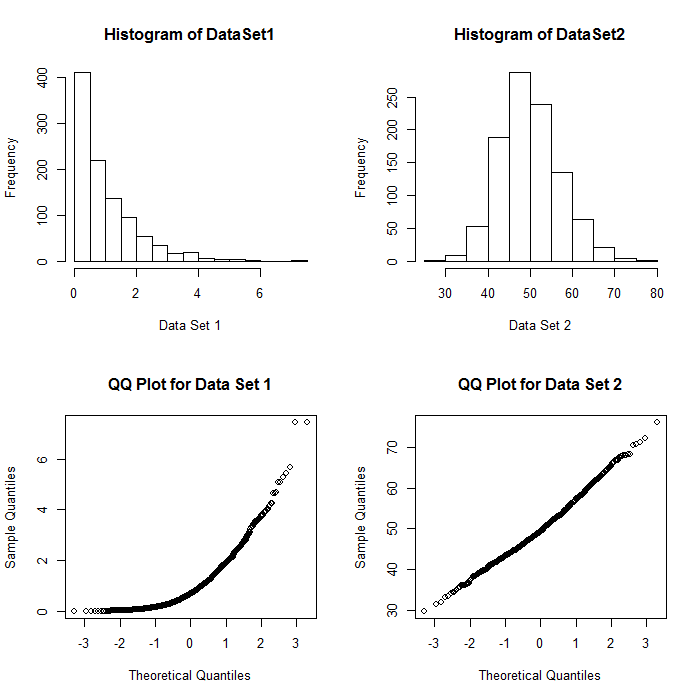
\includegraphics[scale=0.5]{Rplot}
From the histogram and the qq plots, following can be inferred for dataset 1 and dataset 2.
\begin{enumerate}
\item For Dataset 1, the distribution is skewed right, as seen in the qq plot. The distribution does not seem normal and is evident from the proof that mean(0.998600) is far from median(0.692800). The distribution does not show any kind of symmetry.
\item For dataset 2, the distribution seems to be normal, this can be inferred from near straight line in qqplot. The distribution seems to suffer from fat tailed distribution to the right. Since this is a near-normal distribution mean(50) is near to median(49.44). There seems to be a symmetry through the median, however this is not perfect. This goes with the discussion in the class that the practical data sets and models seldom match with the perfect theoretical models and assumptions.
\end{enumerate}
\item Histograms are already available in the previous plot.
\item For the purpose of this homework, only Guassian, Rectangular and Triangular Kernel Density measures are considered.
\\The Kernel Density distribution for dataset 1 is as follows,\\
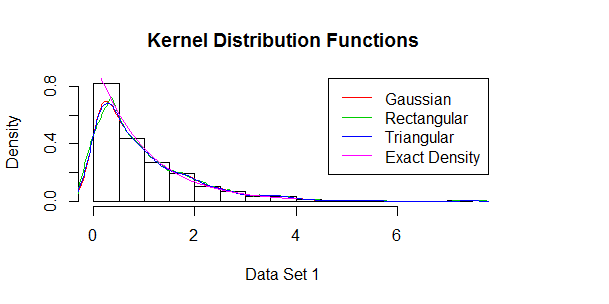
\includegraphics[scale=0.5]{kernel1}
\\The Kernel Density distribution for dataset 2 is as follows,\\
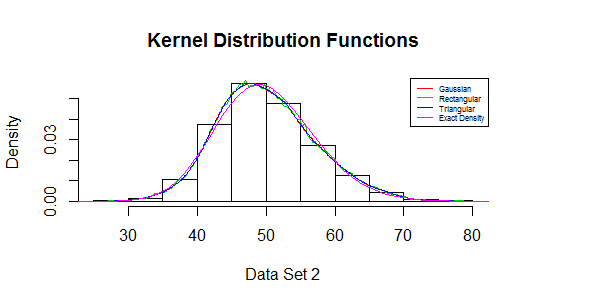
\includegraphics[scale=0.5]{kernel2}
It can be inferred from the plots that for the data set 1, for rectangular method, there is a steep increase initially when compared to the Guassian and Triangular method. However for these data sets, Gaussian Distribution seems the most to represent the function.
\end{enumerate}
\end{enumerate}
\end{document}